% creating appendix
	\appendix
	\chapter{Datenmanagement}
	Dieses Kapitel erläutert einige bedeutende Aspekte der Implementierung des \repag{}en. Diese sind sehr speziell und werden daher nur benötigt, wenn der Quelltext verstanden werden will.
	
	\section{Text-Level}\label{kap_textlevels}
	Da die Konsole eine formatierte Ausgabe erlaubt, wurden sogenannte \emph{Text-Level} eingeführt. Diese lauten (von wichtig zu unwichtig):
	
	\begin{enumerate}
		\item \emph{Fatal}: Das Problem, welches diese Nachricht verursacht, bringt das Programm zum Absturz.
		\item \emph{Error}: Dieses Problem kann nicht ignoriert werden. Das Programm läuft dennoch fort.
		\item \emph{Warning}: Das aufgetretene Problem kann ignoriert werden.
		\item \emph{Information Important}: Der Text beinhaltet eine wichtige Information für den Benutzer.
		\item \emph{Information Casual}: Der Text beinhaltet eine beiläufige Information für den Benutzer, welche dieser nicht unbedingt benötigt.
		\item \emph{Debug}: Der Text dient ausschließlich als Debug-Information. Der Benutzer sollte diese Information nicht sehen.
		\item \emph{Unknown}: Falls kein Text-Level definiert ist oder sonstige Fehler bei dessen Dekodierung auftreten.
	\end{enumerate}
	
	\section{Wichtige Klassen}\label{kap_impCl}
	\paragraph{reportagent.stats.Parameter}
	Repräsentiert einen Datensatz mit sämtlichen Informationen, die zur Darstellung eines Prozessparameters erforderlich sind, \zB{} den Diagramm-Typ. Das zur Klasse zugehörige Attribut \emph{parameterID} definiert klar den Typ des Prozessparameters, \zB{} Fortschritt.\parag{}
	\emph{Hinweis:} Dieses Attribut darf keinesfalls mit dem Attribut \emph{type} verwechselt werden, welches den \emph{Diagramm-Typ} spezifiziert, also \zB{} ein XY-Chart.

	\paragraph{reportagent.stats.ParameterMap}
	Abstrakte Klasse, die Informationen über einzelne Parametertypen enthält, beispielsweise das X-Achsen-Label des Parameters \emph{PCStatus}.

	\paragraph{reportagent.ProtocolRA}
	Interface, welches Konstanten beinhaltet. Diese definieren das Übertragungsprotokoll (siehe Kapitel \ref{kap_protocol}).

	\section{Das Übertragungsprotokoll}\label{kap_protocol}
	Übertragen werden müssen folgende Kommandos:

	\paragraph{REGISTER\_PARAMETER}
	Befehl zur Registrierung eines neuen Prozessparameters beim \repag{}en. Es wird erwartet, dass in der ACLMessage als \emph{ContentObject} ein Objekt des Typs \emph{Parameter} vorliegt.

	\paragraph{UNREGISTER\_PARAMETER}
	Befehl zum Löschen eines Prozessparameters. Wieder wird als \emph{ContentObject} ein Objekt vom Typ Parameter erwartet.

	\paragraph{UPDATE\_PARAMETER}\label{kap_UpdateMsg}
	Befehl zum Update eines Prozessparameters. Die Syntax lautet:

	\begin{lstlisting}[caption={Syntax UPDATE\_PARAMETER},label={lst_syntax_datentag}]
		<parameterID>;<Daten>
	\end{lstlisting}

	wobei der Tag \textit{Daten} frei spezifiziert werden darf. Der Code zur Interpretation dieser Zeile findet sich dabei in der Klasse \emph{reportagent.""behaviours.""Update"-Msg"-Handler}.

	\section{Austausch der Daten}\label{kap_dataman_austausch}
	Dieser Teil beschreibt die Implementierung des Datentransfers zwischen den Agenten. Diese ist sehr spezifisch und bezieht sich direkt auf die in Kapitel \ref{kap_existingPlatform} vorgestellte Beispielplattform, in die der \repag{} eingebettet ist.
	
	\subsection{Sendeseite}
	Für die Verwaltung der Daten ist der \numag{} mit der Klasse \emph{numericagent.InformationManager} ausgestattet. Die Klasse \emph{InformationManager} besitzt die Methode \emph{addParameter(\ldots)}, die den \repag{}en über einen neuen Prozessparameter informiert. Ferner besitzt der \emph{InformationManager} die Methode \emph{update(\ldots)}, die zuerst \emph{addParameter(\ldots)} aufruft, wenn nicht bereits geschehen. Anschließend wird der \repag{} über die neuen Daten informiert.\parag{}
	Da der \calcag{} von \numag{} erbt, steht ihm diese Klasse ebenfalls zur Verfügung. Zu beachten ist, dass im Design davon ausgegangen wurde, dass es von dieser Klasse nur ein Objekt gibt, dies jedoch nicht sichergestellt wurde. Hintergrund ist, dass es mehrere Instanzen des \repag{}en geben kann. Weiter läuft man bei der Programmierung keine Gefahr, mehrere Instanzen der Klasse \emph{InformationManager} zu erzeugen.

	\subsection{Empfangsseite}
	Die Parameter, die neu registriert werden, werden in dem \repag{}en hinterlegt. In der GUI wird ein neuer Tab mit dem entsprechenden Parameter angelegt. Zu beachten ist, dass ein \repag{} mehrere \numag{}en kennen kann und jeder \numag{} mehrere Parameter besitzen kann. Dies ist in der Datenstruktur zur Speicherung der Parameter berücksichtigt, es ergibt sich das Klassendiagramm aus Abbildung \ref{repag_params}.
	\begin{figure}[ht]
		\centering
		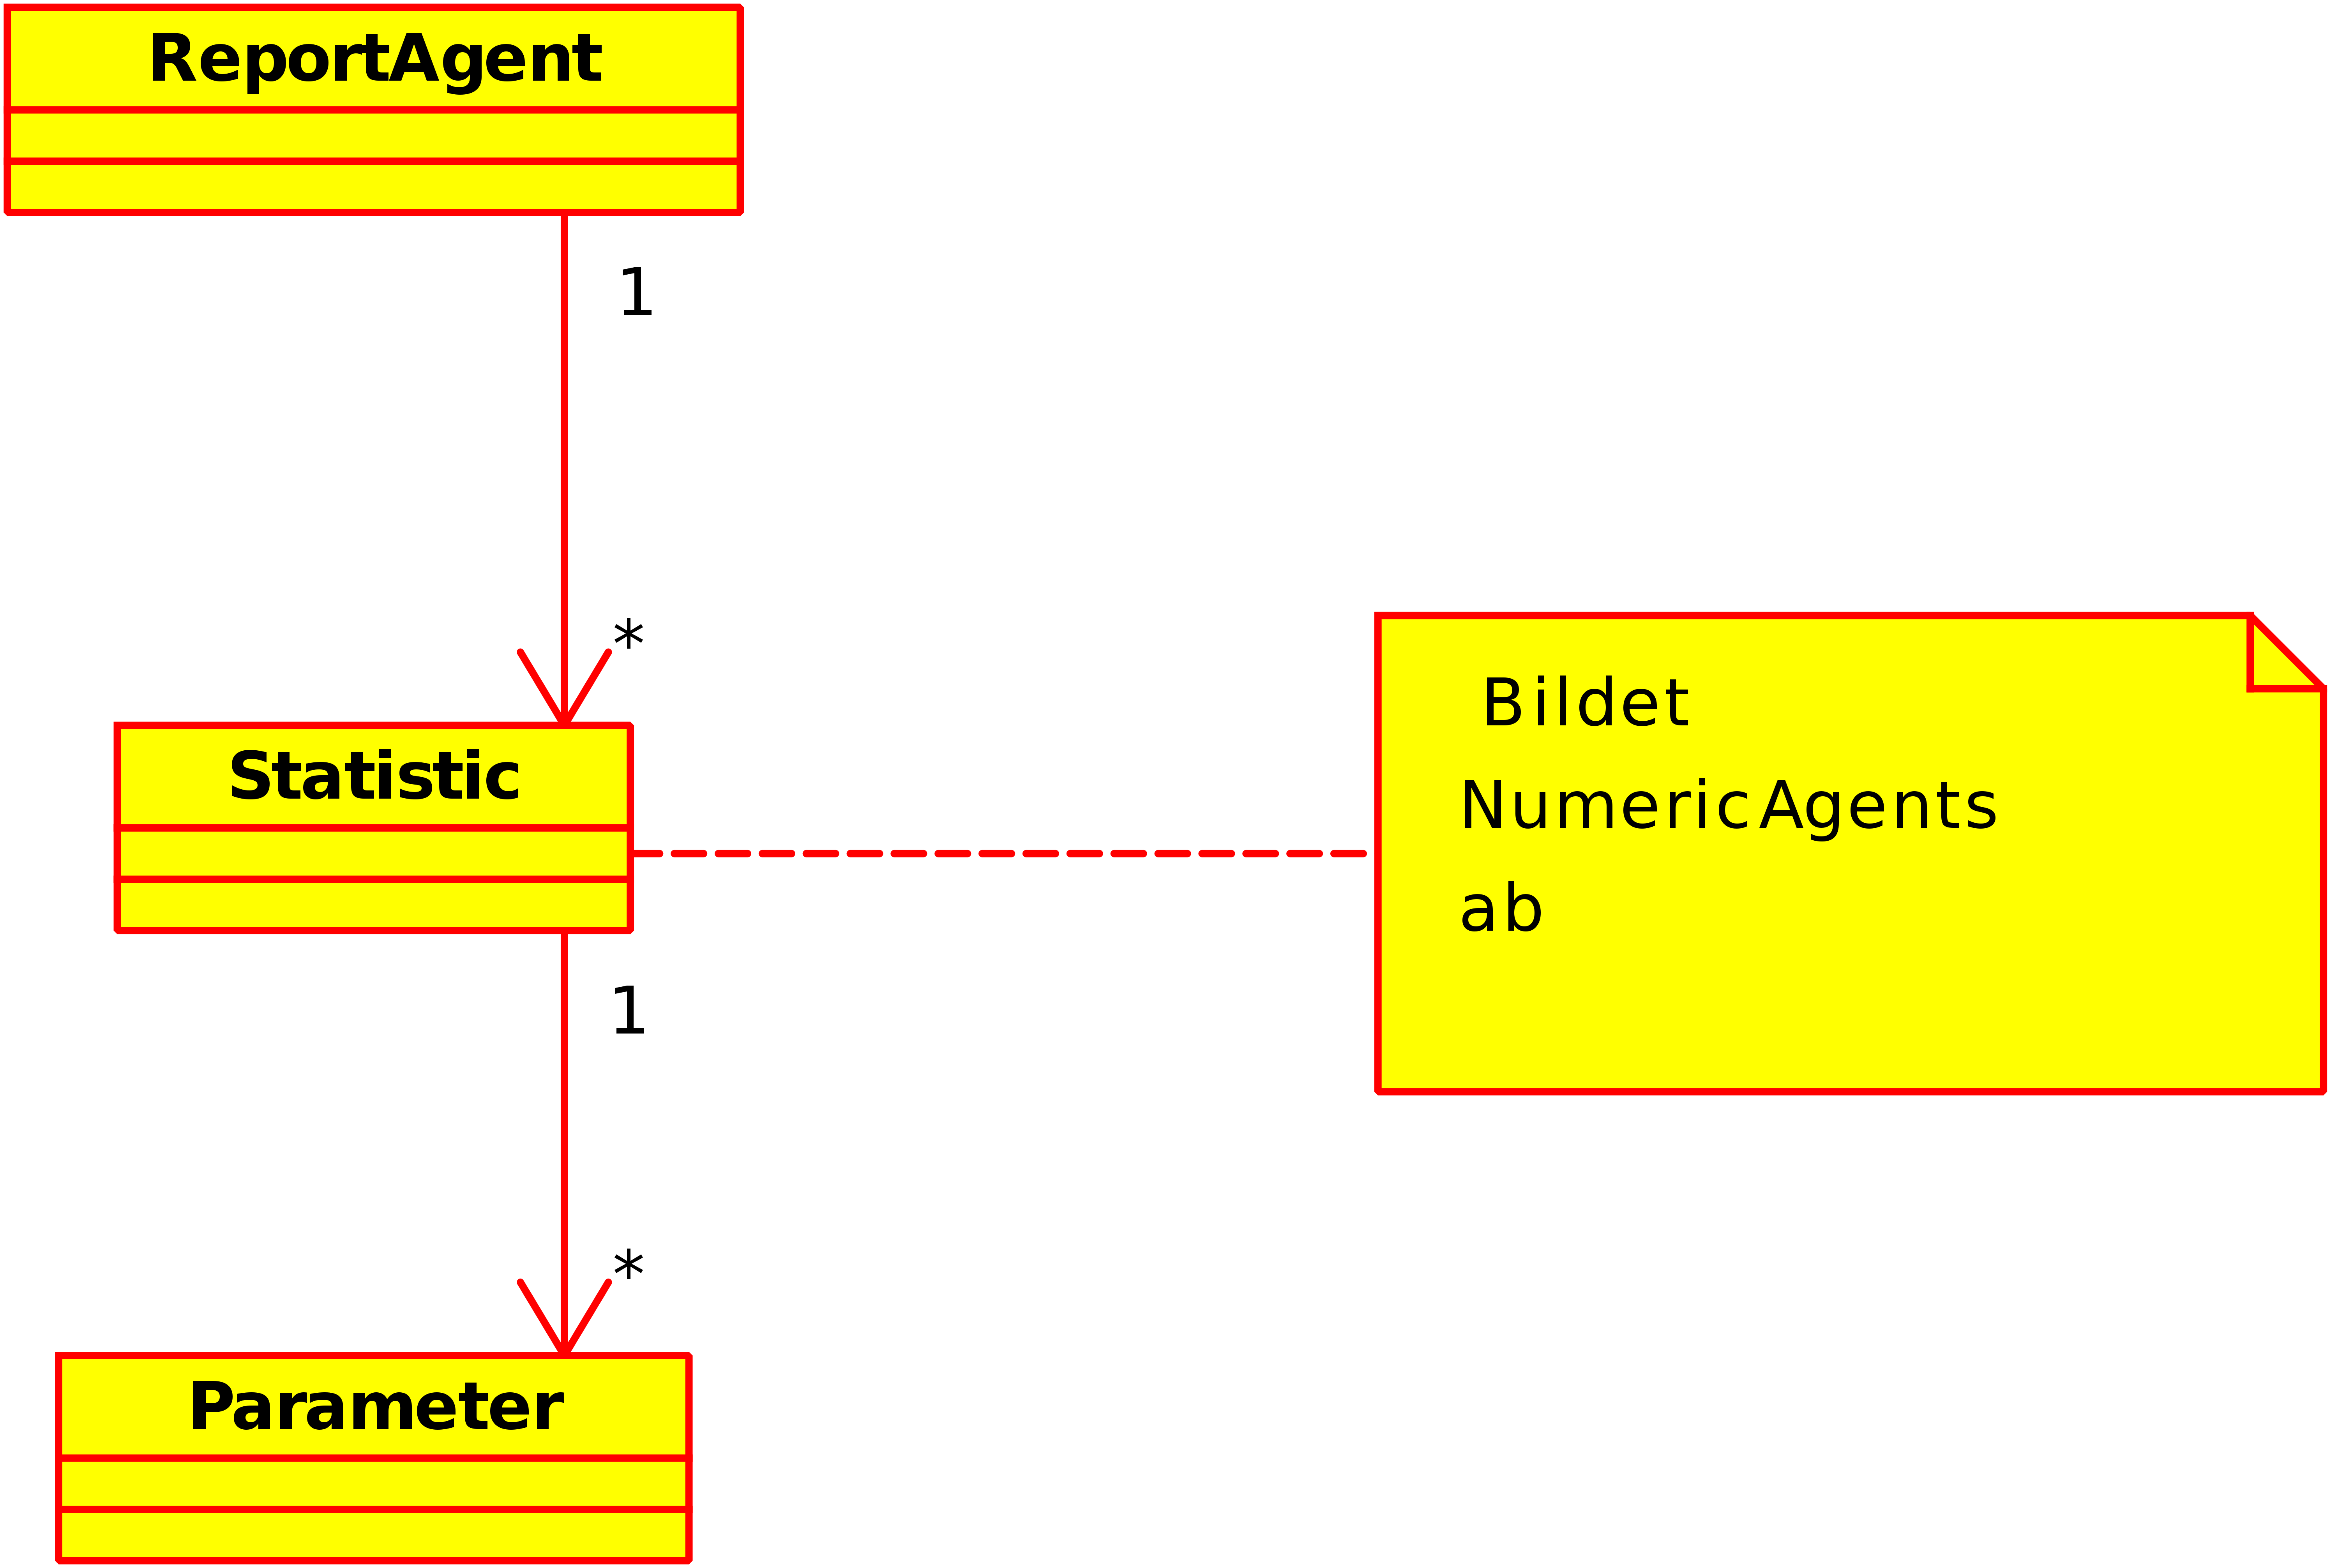
\includegraphics[keepaspectratio=true, width=\textwidth]{res/Klassendiagramm_ReportAgent_Parameterverwaltung.png}
		\caption{Parameterverwaltung des \repag{}en}
		\label{repag_params}
	\end{figure}\parag{}
	Wird nun ein neues Datum empfangen, so wird ein neuer Parameter registriert oder ein bestehender aktualisiert. Die GUI aktualisiert sich in diesem Fall automatisch.
	
	\chapter{Hinzufügen von Prozessparametern}\label{kap_AddParameter}
	Für das nachträgliche Hinzufügen von Parametern in das System müssen lediglich wenige Stellen im Programmtext bearbeitet werden. Diese werden im Folgenden kurz vorgestellt. Da dieses Kapitel als Programmieranleitung gedacht ist, wird für dessen Verständnis Zugang und Verständnis des Quelltextes vorausgesetzt.
	
	\section{Weiterleitung an den \repag{}en}
	Es wird davon ausgegangen, dass die Daten bereits abrufbar sind. Diese müssen an den \repag{}en übergeben werden. Dies geschieht durch die Klasse \emph{numericagent.InformationManager} mit der Methode \emph{addParameter(\ldots)}. Diese ist überladen (siehe \lstlistingname{} \ref{lst_InfoMgr_addParam}).
	\begin{lstlisting}[caption={Auszug aus numericagent.InformationManager},label={lst_InfoMgr_addParam}]	
public void addParameter(Parameter p) {
	...
}

public void addParameter(int paramID) {
	addParameter(new Parameter(paramID));
}
	\end{lstlisting}
	In der einen Version erwartet sie einen Parameter vom Typ \emph{reportagent.stats.Pa\-ra\-me\-ter}, in der anderen einen Parameter vom primitiven Typ \emph{Integer}. Dabei erzeugt die Methode mit dem primitiven Parameter ein neues \emph{Parameter}-Objekt und übergibt dieses an die andere Methode. Obwohl ein Fehlerfall nicht über\-prüf\-bar ist, kann davon ausgegangen werden, dass nach Aufruf dieser Methode das \emph{Parameter}-Objekt korrekt an \repag{} übergeben wurde. Aufgetretene Fehler wird die \emph{update(\ldots)}-Methode beheben.
	
	\section{Parameter}
	Um die \emph{addParameter(\ldots)}-Methode des \emph{InformationManagers} aufrufen zu kön\-nen, wird mindestens eine \emph{parameterID} benötigt (siehe \lstlistingname{} \ref{lst_InfoMgr_addParam}). Diese sollte in der Klasse \emph{Parameter} als Konstanten definiert werden. Dabei ist der Wert in Grenzen frei wählbar -- er sollte zwischen 1 und 2000 liegen. Ein Beispiel ist die Konstante \emph{Parameter.PROGRESS}, die einen Wert von 100 aufweist.\parag{}
	Die genauere Definition des Parameters (Diagramm-Typ, Achsen-Be\-schrif\-tung\-en,\ldots) werden in der Klasse \emph{reportagent.stats.ParameterMap} vorgenommen. Dabei sollten mindestens die Methoden \emph{getParameterType(\ldots)}, \emph{getParameterTitle(\ldots)} und \emph{getParameterDataset(\ldots)} erweitert werden, andernfalls wird eine Warnung ausgegeben. Die Methoden sind alle nach ähnlichem Muster Aufgebaut. Ein Beispiel ist in \lstlistingname{} \ref{lst_ParameterMap_getParameterTitle} zu finden.
	
	\begin{lstlisting}[caption={reportagent.stats.ParameterMap.getParameterTitle()},label={lst_ParameterMap_getParameterTitle}]
public static String getParameterTitle(int parameterID) {
	try {
		switch (parameterID) {
		case Parameter.PROGRESS:
			return "Fortschritt";
			
		case Parameter.MEMORY:
			return "Speicherauslastung";
			
		case Parameter.PCSTATUS:
			return "PC-Status-Monitor";
			
		default:
			handleUnknownParameterError();
			return null;
		}
	} catch (Exception e) {
		return null;
	}
}
	\end{lstlisting}
	
	Hier ist zu erkennen, dass die Methoden als \emph{static} deklariert sind. Die Differenzierung der Parameter erfolgt in einer die Methode bestimmenden \emph{switch}-Verzweigung. Hier muss durch ein weiteres \emph{case}-Statement lediglich der neue Prozessparameter definiert werden. Hierbei ist die \emph{ID} des Prozessparameters, definiert in \emph{reportagent.stats.Parameter}, anzugeben.
	
	\section{Update-Messages}
	Sofern der Prozessparameter aktualisiert werden muss, muss auch die Update-Message \emph{UPDATE\_PARAMETER} definiert werden (siehe dazu Kapitel \ref{kap_UpdateMsg}). Dies geschieht sendeseitig durch einen entsprechenden Aufruf der Methode \emph{update(\ldots)} des \emph{InformationManagers}. Der übergebene Parameter \emph{updateMsg} vom Typ String muss dabei die korrekte Definition des \emph{Daten}-Tags wahren (siehe \lstlistingname{} \ref{lst_syntax_datentag}). Empfangsseitig muss die Methode \emph{action()} der Klasse \emph{reportagent.""behaviours.""Update\-Msg\-Handler} erweitert werden (siehe \lstlistingname{} \ref{lst_UpdateMsgHandler_action}). In der Methode wird zuerst geprüft, ob die Nachricht korrekt ist. Die Interpretation des \emph{Daten}-Tags findet in der großen \emph{switch}-Anweisung am unteren Ende der Methode statt.
	
	\begin{lstlisting}[caption={reportagent.behaviours.UpdateMsgHandler.action()},label={lst_UpdateMsgHandler_action}]
try {
	// Validierung und Vorverarbeitung der Nachricht
	
	switch(p.getParameterID()) {
		// Verarbeitung des Daten-Tags
		// Erweiterung hier!
	}
} catch (Exception e) {
	e.printStackTrace();
}
	\end{lstlisting}
